\chapter{Example Chapter One}

\section{First Section}

\subsection{Subsection One}

\begin{figure}
\centering
\includegraphics[width=0.8\textwidth]{aurora.jpg}
\caption{A figure with a caption}
\label{fig:aurora}
\end{figure}

Figure \ref{fig:aurora} shows a picture.

Citation of a book \cite{hartley2004}.

Let $x$ and $u$ be variables, then:
\begin{equation}
\frac{d}{dx} \left( \int_{0}^{x} f(u)\,du \right) = f(x) ~.
\end{equation}

%\lipsum[1-2]

\subsection{Subsection Two}

\begin{figure}
\centering
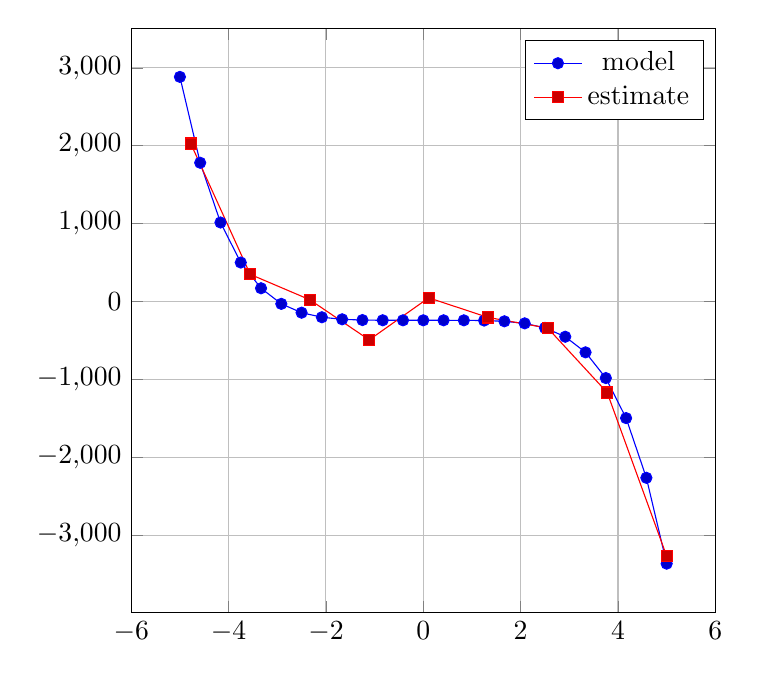
\begin{tikzpicture} \begin{axis}[ height=9cm, width=9cm, grid=major, ] 

\addplot {-x^5 - 242}; \addlegendentry{model} 

\addplot coordinates { (-4.77778,2027.60977) (-3.55556,347.84069) (-2.33333,22.58953) (-1.11111,-493.50066) (0.11111,46.66082) (1.33333,-205.56286) (2.55556,-341.40638) (3.77778,-1169.24780) (5.00000,-3269.56775) }; 
\addlegendentry{estimate} 

\end{axis} 
\end{tikzpicture}
\caption{A tikz plot with a caption}
\label{fig:plot}
\end{figure}

Figure \ref{fig:plot} shows a plot generated with tikz and pgfplots.

%\lipsum[4-5]

\section{Another Section}

\begin{table}
\centering
\begin{tabular}{ l | c || r }
  1 & 2 & 3 \\
  4 & 5 & 6 \\
  7 & 8 & 9 \\
\end{tabular}
\caption{A table with numbers}
\label{tab:numbers}
\end{table}

Numbers are shown in table \ref{tab:numbers}

%\lipsum[6-12]